\section{Mechanic Design} \label{sec:mechanic}
This week the overall mechanical design was discussed. By observing the similar systems, a rude concept of the design was made.  Mechanical design part was divided into two categories: Inner design and Outer design.
Inner design might be problematic since it includes the food and water tank systems. In order to control the amount of the cat food which will flow through food container, the gate should be designed and this gate should effectively cut the food flow. We have think about some gates like using magnets for holding the door or using a system like spinning wheel. However in first case the power of the magnet might not enough for holding the door therefore we have to make some editions in order to make it work. Moreover due to the magnets magnetic field other devices might be suffer. In the second case the spinning wheel might also cause some problems like, it might not rotate due to the friction between food and bucket. Moreover in order to implement it one has to use powerful motor and due to the size of the spinning wheel the overall systems will be huge, which is not desirable for aesthetic and economic reasons. On the other hand we came up with an idea that we can use a systems like ordinary salts have. One can see this on figure \ref{fig:tuzluk}

\begin{figure}
    \centering
    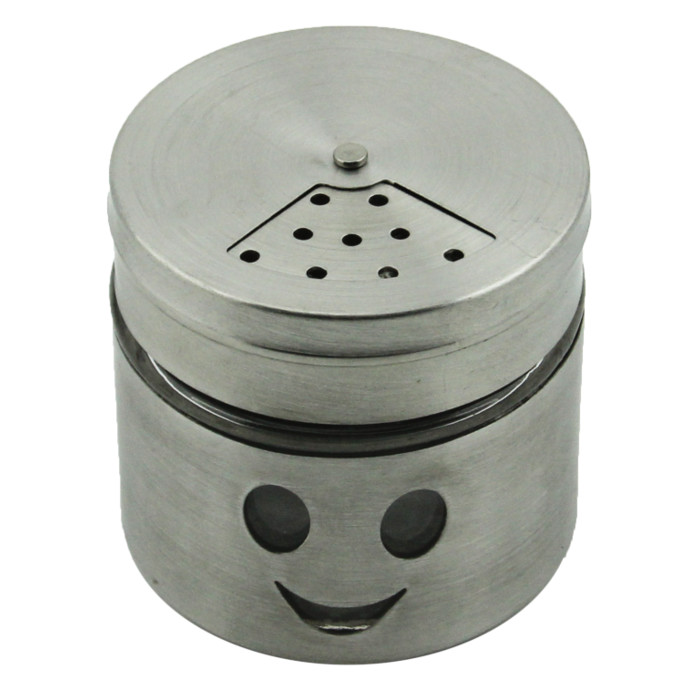
\includegraphics[width=.4\linewidth]{img/Tuzluk.jpg}
    \caption{Salt Cup}
    \label{fig:tuzluk}
\end{figure}

This systems is applicable since one can control the flow of the food by rotating the cover of the salt cup. When two open sides are matched food flows however when one open side matches with a closed side of the cover food flow stops.
Outer design will be handled when the inner design is fixed since, the dimensions of it will be determined by the system which be implemented inside.
